% !TEX program = lualatex
\documentclass[14pt]{extreport}

\usepackage{fontspec}
\setmainfont{Times New Roman}
\setmonofont{Courier New}
\newfontfamily\cyrillicfonttt{Courier New}

\usepackage{polyglossia}
\setmainlanguage{russian}
\setotherlanguage{english}
\gappto\captionsrussian{\renewcommand{\contentsname}{Содержание}}
\gappto\captionsrussian{\renewcommand{\bibname}{Список литературы}}

\usepackage[a4paper,left=30mm,right=10mm,top=20mm,bottom=20mm]{geometry}
\usepackage{indentfirst}
\setlength{\parindent}{1.25cm}
\usepackage{setspace}
\onehalfspacing
\pagestyle{plain}

% Нумерация и содержание до уровня subsubsection
\setcounter{secnumdepth}{3}
\setcounter{tocdepth}{3}

% Формулы
\usepackage{amsmath}

% Рисунки и таблицы
\usepackage{graphicx}
\usepackage{float}
\usepackage{caption}
\captionsetup{labelsep=endash}
\captionsetup[figure]{name=Рисунок}
\captionsetup[table]{position=top, justification=raggedright, singlelinecheck=false}

% Гиперссылки
\usepackage[hidelinks]{hyperref}

\begin{document}

\title{Реферат на тему: \\[0.5cm] \textbf{Искусственный интеллект среди нас}}
\author{Студент: Фролов Андрей Алексеевич \\ Группа: ИВТ-2}
\date{13.09.2026}

\maketitle
\setcounter{page}{2}

\tableofcontents

\chapter*{Введение}
\addcontentsline{toc}{chapter}{Введение}
\textbf{Искусственный интеллект} (ИИ) из научной фантастики превратился
в повседневный инструмент: он подбирает рекомендации, переводит тексты,
пишет код и управляет автомобилями. Вместе с пользой растут и опасения
о том, кто кого контролирует (см. рисунок~\ref{fig:ai}).

Цель реферата~--- кратко рассмотреть основы ИИ, области его применения
и связанные с ним риски.

\begin{figure}[H]
\centering
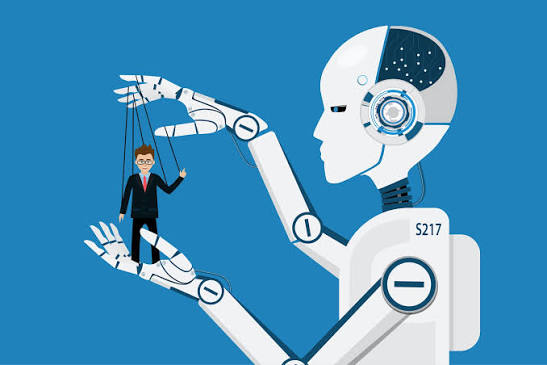
\includegraphics[width=0.5\textwidth]{image.jpg}
\caption{Иллюстрация: ИИ, управляющий человеком}
\label{fig:ai}
\end{figure}

\chapter{Основы искусственного интеллекта}
\section{Понятие ИИ}
Под ИИ понимают системы, способные решать задачи, традиционно требующие
человеческого интеллекта. Основные направления:
\begin{itemize}
\item машинное обучение;
\item обработка естественного языка;
\item компьютерное зрение;
\item робототехника.
\end{itemize}

\section{Нейронные сети}
\subsection{Модель нейрона}
Искусственный нейрон вычисляет взвешенную сумму входов и применяет
функцию активации (формула~\eqref{eq:neuron}):
\begin{equation}
y = \sigma\left(\sum_{i=1}^{n} w_i x_i + b\right),
\label{eq:neuron}
\end{equation}
где $x_i$~--- входы, $w_i$~--- веса, $b$~--- смещение,
$\sigma$~--- функция активации, например сигмоида~\eqref{eq:sigmoid}:
\begin{equation}
\sigma(z) = \frac{1}{1 + e^{-z}}.
\label{eq:sigmoid}
\end{equation}

\subsection{Обучение}
Обучение сети сводится к минимизации функции потерь методом
градиентного спуска~\eqref{eq:gd}:
\begin{equation}
w \leftarrow w - \eta \frac{\partial L}{\partial w},
\label{eq:gd}
\end{equation}
где $\eta$~--- скорость обучения. Этапы обучения:
\begin{enumerate}
\item сбор и разметка данных;
\item прямой проход и вычисление ошибки;
\item обратное распространение ошибки;
\item обновление весов и проверка качества.
\end{enumerate}

\chapter{ИИ в повседневной жизни}
\section{Области применения}
Примеры применения ИИ приведены в таблице~\ref{tab:apps}.

\begin{table}[H]
\caption{Области применения ИИ}
\label{tab:apps}
\centering
\begin{tabular}{|l|l|l|}
\hline
\textbf{Область} & \textbf{Пример} & \textbf{Технология} \\
\hline
Медицина & Анализ снимков & Компьютерное зрение \\
\hline
Транспорт & Беспилотные авто & Обучение с подкреплением \\
\hline
Связь & Голосовые помощники & Распознавание речи \\
\hline
Образование & Чат-боты & Языковые модели \\
\hline
\end{tabular}
\end{table}

\section{Риски и этика}
\subsection{Основные угрозы}
\begin{itemize}
\item утечки персональных данных;
\item предвзятость алгоритмов;
\item дипфейки и дезинформация;
\item вытеснение профессий.
\end{itemize}
\subsubsection{Регулирование}
Правовые нормы в сфере ИИ активно развиваются, например Регламент ЕС
об ИИ~\cite{euact}. Подробнее о теме:
\href{https://ru.wikipedia.org/wiki/Искусственный_интеллект}{статья в Википедии}.

\chapter*{Заключение}
\addcontentsline{toc}{chapter}{Заключение}
ИИ уже прочно вошёл в нашу жизнь (см. таблицу~\ref{tab:apps}). Основой
современных систем служат нейронные сети~\cite{goodfellow, russell},
а главной задачей общества становится их безопасное и этичное использование.

\begin{thebibliography}{9}
\addcontentsline{toc}{chapter}{Список литературы}
\bibitem{russell} Рассел С., Норвиг П. Искусственный интеллект: современный подход.~--- М.: Вильямс, 2006.
\bibitem{goodfellow} Гудфеллоу Я., Бенджио И., Курвилль А. Глубокое обучение.~--- М.: ДМК Пресс, 2018.
\bibitem{euact} Regulation (EU) 2024/1689 (Artificial Intelligence Act).~--- \url{https://eur-lex.europa.eu/eli/reg/2024/1689/oj}.
\end{thebibliography}

\end{document}
